%!TEX root = these.tex

\chapter[Exploitation de VFA pour l'aide à la sélection]{Exploitation du modèle VFA pour la conception de technique de sélection}
\minitoc
\label{chap5}
\cleardoublepage

\section{Introduction}
	Dans ce chapitre, nous présentons premièrement différentes pistes pour concevoir des techniques d'aide à la sélection (ou améliorer des techniques existantes) à l'aide de l'ensemble des enseignements tirés des précédents chapitres, et en particulier du modèle VFA et de son pouvoir de prédiction de la difficulté de sélection d'une cible mobile.
	Deuxièmement, nous exposons un protocole expérimental permettant de valider ce type d'exploitation du modèle VFA, puis nous présentons et analysons les résultats de l'étude empirique menée selon ce protocole.
	Troisièmement, nous proposons une nouvelle technique de sélection, dont la conception s'appuie sur les travaux présentés plus haut dans ce manuscrit.
	Enfin, nous portons un regard critique sur nos résultats, et détaillons une réflexion sur les travaux futurs à mener.
	
\section[VFA : guide pour la sélection de cibles mobiles]{Le modèle VFA comme guide pour les tâches de sélection de cibles mobiles}
	Les résultats que nous avons obtenus et exposés au cours du chapitre~\ref{chap4} montrent, comme de nombreux travaux antérieurs, que la vitesse a un effet déterminant sur les performances de sélection. La première recommandation qui découle de cette observation est de chercher à réduire la vitesse réelle ou effective des cibles mobiles pour en faciliter la sélection.

	Mais comme nous l'avions vu dans le chapitre~\ref{chap4}, la pseudo-entropie, c'est-à-dire le produit AF, a également une influence importante sur les performances de sélection à une vitesse donnée, et permet dans une certaine mesure de les prédire. C'est ce qu'illustre la figure~\ref{fig:tAF} de la section~\ref{sub:previsibility}. Or, l'étude menée sur les périmètres et aires des enveloppes convexes des trajectoires, telle que présentée dans le même chapitre, suggère une plus grande pertinence de la valeur $A\sqrt{F}$, que nous appellerons dorénavant pseudo-entropie subjective, ou PES. Aussi nous apparaît-il judicieux de revisiter la relation entre les performances de sélection et les paramètres VFA, que nous illustrons par la figure~\ref{fig:tAsqrtF}.
	
	\begin{figure}[!htb]
		\centering
		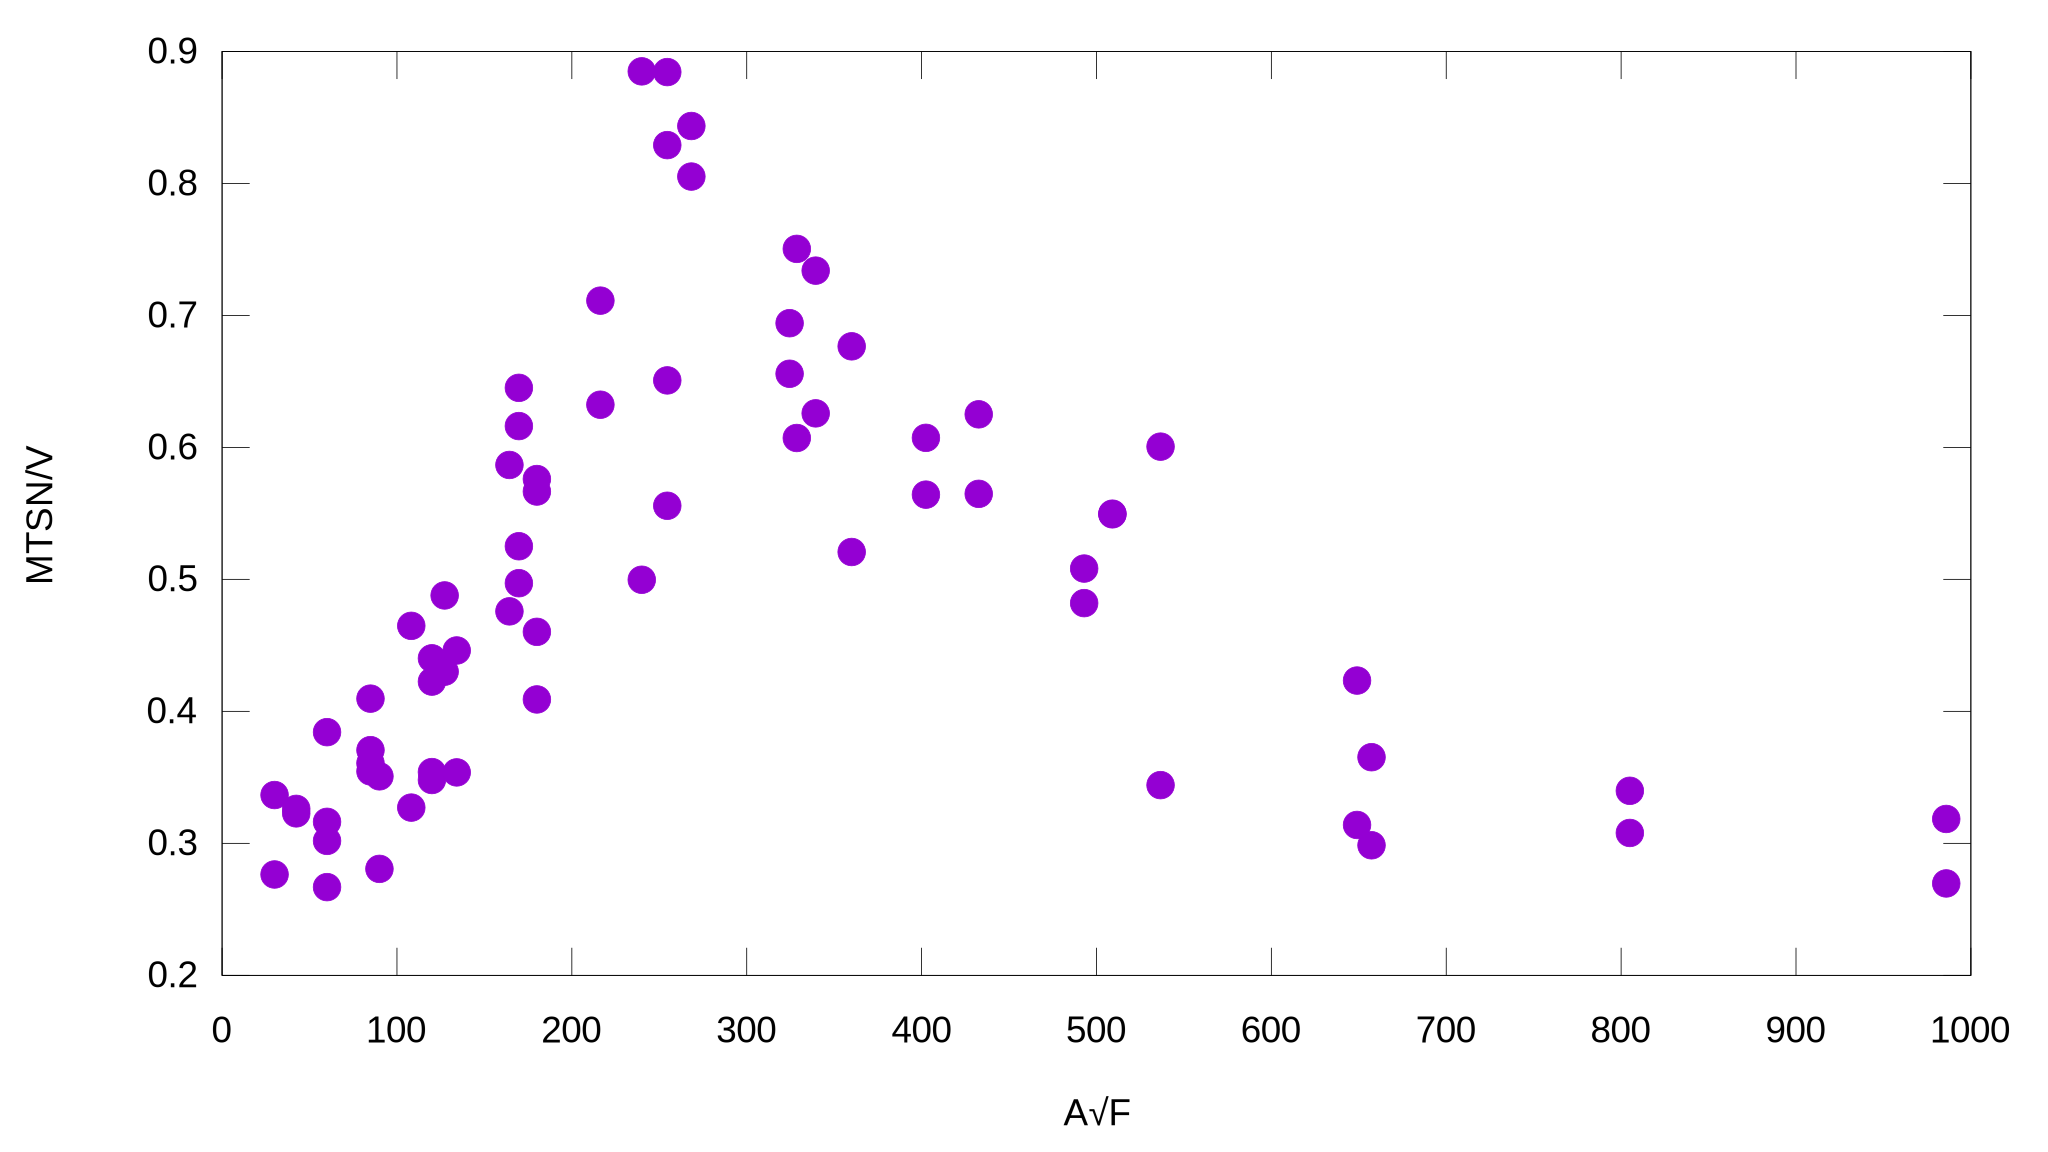
\includegraphics[width=0.8\textwidth]{figures/ch5/asqrtFvTime}
		\caption{Moyennes des temps de sélection normalisés, divisées par la vitesse, en fonction du produit $A\sqrt{F}$, pour des cibles de vitesse moyenne ou rapide.}
		\label{fig:tAsqrtF}
	\end{figure}
	
	Celle-ci nous apprend que lorque la valeur de $A\sqrt{F}$ est autour de 250~$\degree{}Hz^{\frac{1}{2}}$, les temps de sélection sont maximaux. Nous appellerons cette valeur $PES_{max}$. De manière analogue, il est possible de considérer le produit AF, auquel cas cette valeur se trouve autour de 1200~\textdegree{}Hz. Compte tenu des résultats du chapitre 4, il est préférable d'utiliser le produit $A\sqrt{F}$.
	
	Nous pouvons donc en tirer une recommandation pratique simple : chercher à s'éloigner de ces valeurs de référence. Ainsi, la conception d'une application impliquant la sélection de cibles mobiles devrait inclure une phase d'estimation de la pseudo-entropie ou, de manière équivalente et peut-être plus pertinente, de $A\sqrt{F}$. Puis, une phase de réflexion sur les manières dont il serait possible de modifier le comportement des cibles pour s'éloigner de la valeur correspondant à la difficulté maximale.
	
	Concrètement, si la valeur de $A\sqrt{F}$ estimée est inférieure à 250, il faudra chercher à diminuer A ou F ; si elle est supérieure, il faudra chercher à les augmenter. Dans un contexte vidéoludique, par exemple, cela implique de modifier les paramètres de mouvement des objets, si cela n'a pas d'effet délétère sur les mécanismes de jeu. Dans d'autres contextes applicatifs, il n'est pas forcément aisé de modifier le comportement intrinsèque des objets.
	
	Toutefois, cette recommandation pratique vaut autant pour la conception d'applications que pour l'élaboration de techniques d'aide à la sélection. En effet, certaines des techniques de sélection étudiées dans le chapitre~\ref{chap2} sont fondées sur la modification de la taille effective des cibles ou de leur distance au curseur ; lorsqu'il s'agit de cibles mobiles, elles peuvent également agir sur la vitesse, dont nous savons que l'importance est primordiale.
	
	Dans la plupart des contextes applicatifs que nous avons étudiés, la PES d'une cible est généralement en dessous de $PES_{max}$. Pour l'en éloigner encore plus, il faut donc chercher à diminuer A et F. Bien sûr, cette diminution n'est généralement pas incompatible avec l'usage d'une autre technique d'aide à la sélection, comme par exemple le \emph{Bubble Cursor}~\cite{grossman2005bubble}, ou encore \emph{Hook}~\cite{ortega2013hook}.
	
	\subsection{Modification du paramètre F}
	Il est difficile d'imaginer une façon d'augmenter la valeur de F qui ait du sens, à l'exception, peut-être, du choix d'une plus haute fréquence d'échantillonage, lorsqu'il s'agit de données mesurées ou simulées, par exemple pour un enregistrement vidéo, ou une simulation scientifique impliquant des particules.
	
	Toutefois, une option permettant de réduire le paramètre F est d'appliquer un filtrage, par exemple de façon analogue à ce qu'opérerait un filtre passe-bas. La conception d'une telle technique d'assistance à la sélection serait différente selon le degré d'intégration à l'application : avec une intégration forte, il serait possible de modifier directement le comportement des cibles ; avec une intégration faible, il faudrait se contenter d'ajouter un \emph{proxy}, comme le fait la technique \emph{Ghost}~\cite{hasan2011comet}. Ce procédé a par ailleurs l'avantage d'éviter de perdre les informations concernant les positions exactes des cibles potentielles, au prix d'un encombrement visuel accru.
	
	\subsubsection{Filtrage avec limitation à 4~Hz}
	Illustrons notre propos par un exemple concret de technique d'aide à la sélection, fondée sur une limitation de la fréquence de changements de direction à 4~Hz --- ce choix est quelque peu arbitraire, mais informé par les données de la figure~\ref{fig:fEffectPerf}, section~\ref{sub:freqEffect}. Si une cible a un paramètre F dont la valeur intrinsèque est de 32~Hz, un \emph{proxy} de la cible est créé, mais sa position n'est mise à jour que quatre fois par seconde ; les valeurs intérmédiaires étant interpolées. Cette méthode a l'avantage de permettre au \emph{proxy}, dans une certaine mesure, de \og coller \fg{} aux mouvements de la cible réelle, mais de manière moins saccadée, plus prévisible.
	
	Cela se fait toutefois au prix d'une latence inversement proportionnelle à la fréquence d'échantillonage choisie, c'est-à-dire ici $\frac{1}{4}~s = 250~ms$. Naturellement, il est possible de réduire cette latence en augmentant la fréquence d'échantillonage, ce qui a l'inconvénient de diminuer l'efficacité de la technique.
	
	Cette façon de filtrer les positions des cibles permet de conserver des points en commun avec la trajectoire initiale, et donc de ne pas trop en modifier l'étendue ; nous reviendrons sur ce point plus loin avec des illustrations.
	
	Il est important de noter (et encore une fois, la figure~\ref{fig:fEffectPerf} l'illustre) que la réduction de la fréquence permet d'améliorer les performances, mais que cette réduction est moins perceptible lorsque le paramètre A est particulièrement grand. 

	\subsection{Modification du paramètre A}
	Dans ces cas-là, il peut être plus judicieux de chercher à diminuer ce dernier --- là encore, il paraît difficile de chercher à l'augmenter de manière sensée. La réduction du paramètre A est peut-être plus délicate que celle de F, attendu qu'elle ne se prête pas à un filtrage temporel.
	
	Certes, s'il est possible de modifier directement le comportement des objets, alors la réduction de A peut s'avérer possible dans certaines circonstances, à condition qu'elle n'ait pas d'impact trop négatif sur l'application concernée.
	
	\subsubsection{Report de la pseudo-entropie sur F}
	Pour rappel, les paramètres A et F ne sont pas égaux dans leur influence sur les performances de sélection, puisque c'est la racine carrée de F dont l'influence est primordiale, et non F lui-même. Par conséquent, il peut être judicieux de diminuer A et d'augmenter F proportionnellement, pour compenser, et maintenir une pseudo-entropie constante, si le contexte applicatif l'exige.
	
	Supposons en effet une cible dont la pseudo-entropie subjective est la \og pire \fg{} possible, soit $A\sqrt{F} = PES_{max} = 250$, avec $A = 50~; F = 25~; \sqrt{F} = 5~; AF = 1250$.
	
	S'il on veut conserver la même quantité de désordre sur une durée donnée, il faut maintenir le produit AF constant à 250. Pour ce faire, nous pouvons, par exemple, diviser A par 2, et multiplier F par le même nombre, ce qui aboutit à la situation suivante : $A = 25~; F = 50~; \sqrt{F} \approx 7,07$ ; d'où $A\sqrt{F} \approx 176,78$, soit une diminution de la PES qui l'éloigne de $PES_{max}$.
	
	Naturellement, l'effet est d'autant plus fort que le facteur choisi est élevé ; ainsi, avec 5, nous obtenons les valeurs suivantes : $A = 10~; F = 125~; \sqrt{F} \approx 11,18~; A\sqrt{F} \approx 111,80$. La figure~\ref{fig:tAsqrtF} montre que pour ces valeurs de PES, les performances de sélection sont bien meilleures que pour $PES_{max}$. Néanmoins, tous les dispositifs d'affichage ne sont pas capables d'atteindre de telles fréquences, ce qui limite la portée de cette approche.
	
	\subsubsection{Limitation de A avec compensation ultérieure}
	Une autre option consiste à imposer une limite ferme à la cible (ou à son \emph{proxy}) et à chercher à compenser à chaque nouveau changement de direction. Supposons par exemple une borne de 30\textdegree{} imposée au paramètre A, et un proxy représentant chaque cible. Pour une cible donnée, si son vecteur vitesse subit à un instant $t$ une rotation de plus de 30\textdegree{}, son \emph{proxy} ne voit son vecteur vitesse tourner que de 30\textdegree{}. Lors du prochain changement de direction du vecteur vitesse, celui du proxy est alors ajusté non pas de manière à correspondre à la nouvelle rotation subie par le vecteur vitesse réelle, mais de manière à orienter le proxy dans la direction de la cible qu'il représente, pour compenser le décalage induit par l'imposition d'une borne sur A. Cette compensation se fait néanmoins toujours avec au plus une rotation de 30\textdegree{}.
	
	Cette opération est possible sans que la distance entre la cible et son \emph{proxy} ne diverge, car les changements de direction limitent la distance totale parcourue par un objet sur une période et à une vitesse données, attendu que c'est en allant tout droit que l'on s'éloigne le plus de son point de départ.
	
	Néanmoins, selon le paramètre A intrinsèque de la cible, et selon la borne imposée, le comportement du \emph{proxy} peut-être plus ou moins déconnecté de celui de la cible potentielle qu'il représente ; aussi la prudence est-elle de mise lorsque cette technique est mise en œuvre, et il est probablement souhaitable d'éviter d'avoir un écart trop important entre la valeur originelle de A et la borne choisie. Il est toutefois possible de combiner cette imposition de borne avec le report de l'entropie sur F.
	
	\subsubsection{Filtrage par moyenne mobile}
	La moyenne mobile constitue un type de filtrage passe-bas assez classique. Elle consiste, pour une largeur L, à remplacer chaque valeur $x_{i}$ rencontrée dans une série par la moyenne d'un échantillon de L valeurs centré sur $x_{i}$. Là encore, une latence est introduite par le procédé, et elle est proportionnelle à L. Il serait probablement mal aviser de chercher à lisser ainsi les angles de rotation du vecteur vitesse d'une cible, car cela introduirait un décalage potentiellement divergent entre la position de la cible et celle de son \emph{proxy}.
	
	Cependant, il est possible d'appliquer un tel filtrage aux positions mêmes de la cible. Dans ce cas, F demeure inchangé, mais A est diminué de fait --- ou plus rigoureusement, la valeur moyenne des angles de rotation du vecteur vitesse est diminuée, car nous avons défini A comme la borne supérieur de ces angles, et la diminution de cette borne est moins évidente.
	
	Ici et comme avec d'autres méthodes de filtrage évoquées plus haut, un compromis entre le \og pouvoir \fg{} de lissage et la latence proportionnelle à L doit être trouvé de manière \emph{ad hoc}, selon le contexte applicatif.
	
	
	\subsection{Utilisation dynamique des proxies}
	Comme nous le précisions notamment dans la section~\ref{sub:techAug} qui évoque les techniques fondées sur l'augmentation des cibles, cette approche a l'inconvénient majeur d'accroître l'encombrement visuel, généralement d'un facteur deux lorsqu'elle implique l'utilisation de \emph{proxies}. Toutefois, il est tout à fait possible de mitiger cet impact en combinant cette approche avec de la prédiction intentionnelle. Par exemple, la technique \emph{Hook}~\cite{ortega2013hook} maintient en permanence une liste des N cibles potentielles les plus proches du curseur, où N est un entier naturel paramétrable. Ce procédé très simple pourrait être utiliser pour restreindre l'usage des \emph{proxies} : seules les N cibles en question en seraient accompagnées, les autres étant jugées trop loin du curseur pour être visées par l'utilisateur.
	
	Naturellement, selon le contexte, d'autres approches pourraient être pertinentes, comme celle d'\emph{IntenSelect}~\cite{de2005intenselect}, par exemple, fondée sur un principe similaire, mais appliqué à des rayons lancés depuis un périphérique de saisie, plutôt qu'à un curseur ponctuel. Quelle que soit l'approche exacte choisie, si le nombre de \emph{proxies} est beaucoup plus petit que le nombre total de cibles potentielles, l'encombrement visuel ajouté est faible, potentiellement inférieur à 10~\%{}, voire moins si l'on opte pour des \emph{proxies} partiellement transparents, par exemple.

	
\clearpage